\documentclass[conference]{IEEEtran}
\IEEEoverridecommandlockouts

\usepackage{cite}
\usepackage{amsmath,amssymb,amsfonts}
\usepackage{algorithmic}
\usepackage[utf8]{inputenc}
\usepackage{multirow}
\usepackage{booktabs}
\usepackage{tabularx}
\usepackage{graphicx}
\usepackage{textcomp}
\usepackage{xcolor}
\usepackage[english]{babel}
\usepackage{url}
\usepackage{tikz}
\usetikzlibrary{positioning,arrows.meta,shapes.geometric}

\def\BibTeX{{\rm B\kern-.05em{\sc i\kern-.025em b}\kern-.08em
    T\kern-.1667em\lower.7ex\hbox{E}\kern-.125emX}}

\begin{document}

\title{EEG-Based Coffee Aroma Discrimination Using Machine Learning to Decode Brain Responses to Olfactory Stimuli\\
}

\author{%
  \IEEEauthorblockN{%
    Le Trung Kien\textsuperscript{1},
    Do Viet Dat\textsuperscript{1},
    Tran Thi Tram Anh\textsuperscript{1},
    Phan Phuong Linh\textsuperscript{1},\\
    Tran Xuan Tien\textsuperscript{2},
    Dong Anh Quoc\textsuperscript{2},
    Bui Huy Kien\textsuperscript{1},
    Satoshi Honda\textsuperscript{1,*}%
  }
  \IEEEauthorblockA{%
    \textsuperscript{1}\,Vietnam Japan University, Vietnam National University, Hanoi, Vietnam\\
    \textsuperscript{2}\,Hanoi University of Science and Technology, Hanoi, Vietnam\\
    \textsuperscript{*}\,Corresponding author: honda.s@vju.ac.vn%
  }%
}

\maketitle

\begin{abstract}
Coffee aroma drives consumer preference and market value, but sensory panels are subjective and electronic noses describe chemistry rather than perception. We tested whether scalp EEG with classical machine learning can discriminate \textit{Coffea arabica} from \textit{Coffea canephora} (Robusta) aromas at the single trial level. Twenty volunteers were recorded with a 16 channel KT88 amplifier at 100~Hz over 45 sniff trials per session (15 Arabica, 15 Robusta, 15 odourless air). After band pass filtering, common average referencing, and artefact rejection, we classified three second epochs with logistic regression, an RBF SVM, and a random forest under strict leave one subject out (LOSO) evaluation. A transparent data quality audit identified hardware clipping ($\geq 2.3\,\%$ samples railed at $\pm 204.8\,\mu$V) in 11 of 18 acquired recordings, indicating contamination by interference whose amplitude exceeds physiological scalp EEG by a factor of four or more, with broadband elevation of the power spectrum; those recordings were excluded to avoid a per subject confounder, leaving 238 odor epochs from eight participants. The best random forest reached an accuracy of 0.546 (AUC 0.553) on band power features; the highest configuration of a 72 cell feature search (engineered superset, random forest) reached a balanced accuracy of 0.588. An easier coffee versus air contrast peaked at 0.538 and a pseudo subject control confirmed the result is not a fold size artefact. The only systematically above chance result was within subject three level classification of sensory ratings (balanced accuracy up to 0.48, chance 0.33). We release the dataset, the pipeline, and a calibrated reference point for subject independent EEG decoding of closely related natural odors.
\end{abstract}

\begin{IEEEkeywords}
EEG, olfactory perception, coffee aroma, machine learning, brain--computer interface.
\end{IEEEkeywords}

\section{Introduction}
Coffee is one of the most traded agricultural commodities worldwide, and the two dominant species \textit{Coffea arabica} and \textit{Coffea canephora} (Robusta) command very different prices, with partial substitution being a recurring form of adulteration \cite{ico2023,cardoso2025}. Quality assurance still relies on trained sensory panels and instrumental methods such as GC--MS or electronic noses \cite{bressanello2017,pardo2002}, both of which describe either human judgement or chemistry, but not the cortical response that ultimately defines perceived aroma. Scalp EEG offers a complementary, non invasive window: odors modulate band power and chemosensory event related potentials over fronto-temporal sites \cite{pause2000,kroupi2014}, and recent multivariate decoding work shows that odor information is available in EEG within the first half second of stimulus onset \cite{iravani2022}.

Machine learning has accelerated single trial EEG decoding, with band power features and linear or kernel classifiers as the classical baseline \cite{lotte2018} and compact convolutional networks such as EEGNet \cite{lawhern2018} as a modern alternative. Several groups have reported above chance odor classification, but almost always under within subject splits and between highly dissimilar odorants \cite{kroupi2014,aydemir2017,hou2025}. Whether EEG carries information about closely related natural odors that generalises across participants --- the realistic deployment setting for an aroma decoder --- remains open. Closely related work on coffee specifically has focused on group level oscillatory changes during inhalation \cite{tanaka2024}, not on subject independent classification of species.

This paper addresses that gap with three contributions. First, we collect and release the first 16 channel EEG dataset of Arabica versus Robusta sniffing under a controlled protocol. Second, we benchmark logistic regression, an RBF SVM, and a random forest on spectral band power features and on five additional engineered feature families under strict LOSO evaluation, and we report honest chance level results. Third, we document a hardware clipping artefact in a contiguous block of eleven recordings and show how omitting the corresponding data quality audit would have inflated cross subject accuracy through a per subject confounder rather than genuine olfactory neural activity.

\section{Materials and Methods}

Figure~\ref{fig:pipeline} summarises the end-to-end analysis pipeline from raw EEG to LOSO classification metrics.

\begin{figure}[ht]
  \centering
  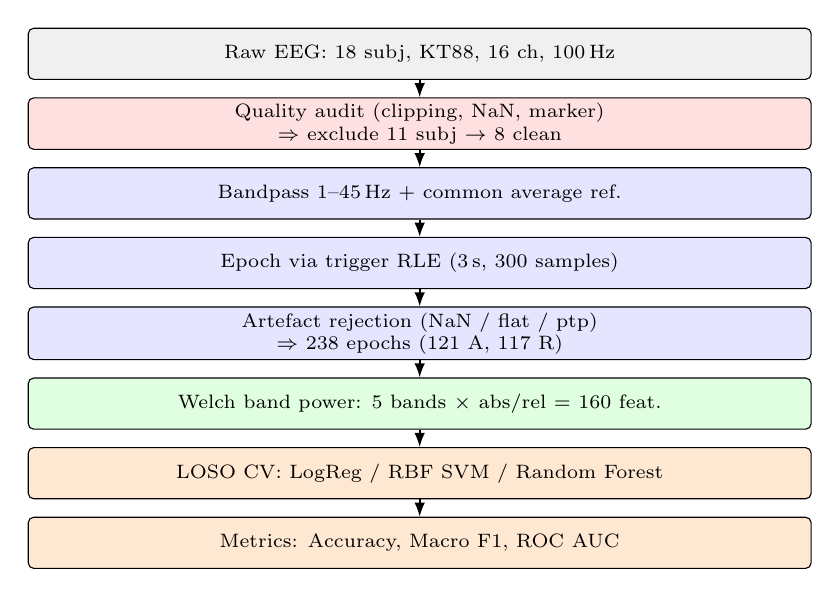
\begin{tikzpicture}[
    node distance=2.2mm,
    block/.style={draw,rounded corners=2pt,minimum width=0.82\columnwidth,minimum height=6.5mm,align=center,font=\scriptsize,inner sep=2pt},
    raw/.style={block,fill=gray!12},
    qa/.style={block,fill=red!12},
    pre/.style={block,fill=blue!10},
    feat/.style={block,fill=green!12},
    cls/.style={block,fill=orange!18},
    arr/.style={-{Latex[length=1.8mm]},semithick}
  ]
    \node[raw] (r) {Raw EEG: 18 subj, KT88, 16 ch, 100\,Hz};
    \node[qa,below=of r] (q) {Quality audit (clipping, NaN, marker)\\$\Rightarrow$ exclude 11 subj $\to$ 8 clean};
    \node[pre,below=of q] (p) {Bandpass 1--45\,Hz + common average ref.};
    \node[pre,below=of p] (e) {Epoch via trigger RLE (3\,s, 300 samples)};
    \node[pre,below=of e] (a) {Artefact rejection (NaN / flat / ptp)\\$\Rightarrow$ 238 epochs (121 A, 117 R)};
    \node[feat,below=of a] (f) {Welch band power: 5 bands $\times$ abs/rel = 160 feat.};
    \node[cls,below=of f] (m) {LOSO CV: LogReg / RBF SVM / Random Forest};
    \node[cls,below=of m] (s) {Metrics: Accuracy, Macro F1, ROC AUC};
    \foreach \x/\y in {r/q,q/p,p/e,e/a,a/f,f/m,m/s}
      \draw[arr] (\x) -- (\y);
  \end{tikzpicture}
  \caption{Analysis pipeline. Red: data quality gate; blue: preprocessing; green: features; orange: evaluation.}
  \label{fig:pipeline}
\end{figure}

\subsection{Participants, Stimuli, and Acquisition}
Twenty volunteers were recruited; two (P002, P008) withdrew before the session, leaving 18 complete datasets. All participants reported normal olfaction, had abstained from food and strongly flavoured drinks for at least two hours before recording, and gave written informed consent under a protocol approved by the institutional ethics board. Stimuli were freshly ground beans of \textit{Coffea arabica} and \textit{Coffea canephora} from the same supplier, roasted to a medium level on the same day. Each session presented 15 Arabica, 15 Robusta, and 15 odourless air trials in a pseudo random order, drawn from a per subject canonical sequence stored separately from the EEG recording. Every trial comprised a two second baseline, a three second deep sniff, and an inter stimulus interval of at least 20~s \cite{kroupi2014,kobal1981}. Each category was mapped to five integer codes identifying the physical vial used (Table~\ref{tab:codes}); for the present binary task only the Arabica and Robusta codes were retained. The single-trial timeline is shown in Fig.~\ref{fig:protocol}.

\begin{figure}[ht]
  \centering
  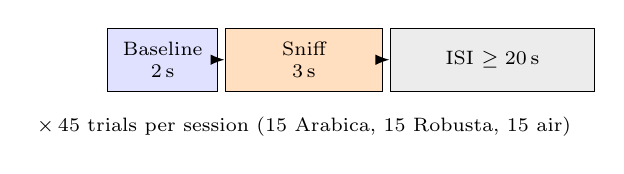
\begin{tikzpicture}[
    seg/.style={draw,minimum height=8mm,align=center,font=\scriptsize,inner sep=2pt},
    arr/.style={-{Latex[length=1.8mm]},semithick}
  ]
    \node[seg,fill=blue!12,minimum width=14mm]  (b) {Baseline\\2\,s};
    \node[seg,fill=orange!25,minimum width=20mm,right=0.8mm of b] (s) {Sniff\\3\,s};
    \node[seg,fill=gray!15,minimum width=26mm,right=0.8mm of s]   (i) {ISI $\geq 20$\,s};
    \node[font=\scriptsize,below=2mm of s] (rep) {$\times\,45$ trials per session (15 Arabica, 15 Robusta, 15 air)};
    \draw[arr] (b.east) -- (s.west);
    \draw[arr] (s.east) -- (i.west);
  \end{tikzpicture}
  \caption{Single-trial timeline. Stimulus order is pseudo-random per subject.}
  \label{fig:protocol}
\end{figure}

EEG was recorded with a Contec KT88 amplifier in a 16 channel configuration (Fp1, Fp2, F3, F4, C3, C4, P3, P4, O1, O2, F7, F8, T3, T4, T5, T6; international 10--20 system \cite{jasper1958}) at 100~Hz, 12~bit ADC, full scale $\pm 204.8\,\mu$V. Two ECG channels were discarded. Electrode impedances were kept below 10~k$\Omega$ and the trigger channel was sampled synchronously with the EEG.

\begin{table}[ht]
  \centering
  \caption{Stimulus categories and trigger codes.}
  \label{tab:codes}
  \footnotesize
  \begin{tabular}{p{0.30\columnwidth} p{0.10\columnwidth} p{0.42\columnwidth}}
    \toprule
    \textbf{Category} & \textbf{Label} & \textbf{Integer codes} \\
    \midrule
    Control (odourless air) & C0 & 712, 238, 759, 869, 562 \\
    \textit{Coffea arabica}    & C1 & 981, 633, 902, 598, 733 \\
    \textit{Coffea canephora}  & C2 & 585, 597, 200, 558, 692 \\
    \bottomrule
  \end{tabular}
\end{table}

\subsection{Data Quality Audit}
Before any signal processing, every recording was passed through an automated audit that checked sampling regularity, flat channels (standard deviation below 0.5~$\mu$V), and hardware saturation (fraction of samples whose absolute amplitude exceeded 204.0~$\mu$V, just below the $\pm 204.8\,\mu$V amplifier rail). The audit revealed a bimodal distribution of saturation (Fig.~\ref{fig:clipping}): participants P003--P013 showed 2.3\,\% to 17\,\% saturated samples (139{,}725--1{,}110{,}804 per recording), while the remaining seven recordings stayed below 0.4\,\%.

Clipping at the $\pm 204.8\,\mu$V rail is not a cosmetic amplitude issue: physiological scalp EEG typically lives within $\pm 50\,\mu$V \cite{lotte2018}, so a signal that pins the rail must be dominated by extra-cerebral interference --- electrode pops, motion, EMG, or amplifier saturation noise --- whose amplitude exceeds the brain signal by a factor of four or more. Figure~\ref{fig:rawpsd} contrasts an eight-second window of F3 in a clean (P001, $\pm 20\,\mu$V) and a clipped (P006, rail-pinned) subject; the clipped Welch PSD is broadband-elevated by $1.3\times$--$2.0\times$ across the theta, alpha, beta, and gamma bands. Because non-linear clipping injects harmonic distortion across all bands and is structured by participant, it acts as a per-subject covariate that a LOSO classifier could exploit instead of the odor label. The eleven affected subjects were therefore excluded before any modelling, leaving a clean cohort of eight (P001, P014--P020). Two additional findings --- two trailing all-NaN rows at the end of P014's recording, which would otherwise propagate through the zero-phase filter, and a manual marker entry mismatch for P019, in which the EEG trigger channel disagreed with the canonical stimulus sequence --- were handled by dropping the affected rows at load time and by labelling epochs from the canonical sequence rather than from the EEG trigger.

\begin{figure*}[ht]
  \centering
  \includegraphics[width=0.95\textwidth]{fig_4_5_raw_psd.png}
  \caption{Raw signal and Welch PSD on F3. (a) Clean P001, $\pm 20\,\mu$V. (b) Clipped P006 saturating at the $\pm 204.8\,\mu$V rail. (c) PSD: P006 broadband-elevated above P001 across 4--45\,Hz.}
  \label{fig:rawpsd}
\end{figure*}

\begin{figure*}[ht]
  \centering
  \includegraphics[width=0.95\textwidth]{fig_4_3_clipping_evidence.png}
  \caption{Hardware clipping evidence on F3. (a) Amplitude histogram. (b) Raw P006 trace. (c) Per-subject saturation rate; red = excluded.}
  \label{fig:clipping}
\end{figure*}

\subsection{Preprocessing, Features, and Classifiers}
Each continuous recording was band pass filtered (4th order Butterworth, 1--45~Hz, zero phase forward backward) before epoch extraction to avoid edge artefacts inside the analysis window \cite{lotte2018}, then common average referenced \cite{mcfarland1997}. Odor epochs were extracted by run length encoding of the trigger channel: every Arabica or Robusta segment of exactly 300 samples was kept. An epoch was rejected if it contained a non finite value, a flat channel (std $< 0.5\,\mu$V), or any channel whose peak to peak amplitude exceeded the adaptive 99th percentile of the epoch level peak to peak distribution. After rejection, the final dataset contained 238 epochs (121 Arabica, 117 Robusta) over the eight clean subjects.

The primary feature set was Welch \cite{welch1967} band power on five canonical bands (delta 1--4, theta 4--8, alpha 8--13, beta 13--30, gamma 30--45~Hz) in absolute and relative form, yielding 160 features per epoch. A feature search additionally evaluated five families: time domain statistics (128 features), Hjorth parameters (48), 2~Hz narrow band power (256), three window temporal band power (480), and an engineered superset (912) selectable via a mutual information criterion at $k \in \{20, 40, 80, \text{all}\}$. Three classifiers were benchmarked: L2 regularised logistic regression, an RBF SVM with probabilistic outputs, and a random forest with 300 class balanced trees. Each model was wrapped in a pipeline of standard scaling, optional feature selection, and classification, with hyperparameters fixed at the scikit learn defaults \cite{pedregosa2011} to avoid leakage through per fold tuning.

Evaluation followed strict leave one subject out cross validation: on each of the eight folds, the held out subject's epochs are predicted by a model fit only on the other seven. We report accuracy, balanced accuracy, macro F1, and ROC AUC; chance level for the two class problems is 0.5 and for the three level sensory classification of Section~\ref{sec:sensory} it is 1/3. The full source code, pipeline, and unit tests will be released with the camera ready version.

\section{Results}
All numbers are taken directly from the artefacts written by the pipeline. The clean cohort contributes 238 epochs distributed as P001=30, P014=31, P015=30, P016=29, P017=29, P018=30, P019=30, P020=29; Arabica vs Robusta are balanced at 121 / 117.

\subsection{Arabica versus Robusta}
On the 160 dimensional band power feature set (Table~\ref{tab:loso-bp}, Fig.~\ref{fig:bars}), all three classifiers stayed within five percentage points of the 0.5 chance level: random forest 0.546 / 0.546 / 0.553 (accuracy / macro F1 / ROC AUC), RBF SVM 0.513 / 0.507 / 0.466, logistic regression 0.466 / 0.465 / 0.496.

\begin{table}[ht]
  \centering
  \caption{LOSO metrics on band power features.}
  \label{tab:loso-bp}
  \footnotesize
  \begin{tabular}{l r r r}
    \toprule
    \textbf{Model} & \textbf{Accuracy} & \textbf{Macro F1} & \textbf{ROC AUC} \\
    \midrule
    Logistic regression & 0.466 & 0.465 & 0.496 \\
    SVM (RBF)           & 0.513 & 0.507 & 0.466 \\
    Random forest       & \textbf{0.546} & \textbf{0.546} & \textbf{0.553} \\
    \bottomrule
  \end{tabular}
\end{table}

\begin{figure}[ht]
  \centering
  \includegraphics[width=\columnwidth]{fig_6_1_arabica_robusta_bars.png}
  \caption{LOSO accuracy on band power features. Error bars: SD across the eight folds; dashed line: chance (0.5).}
  \label{fig:bars}
\end{figure}

The feature search across six families, three classifiers, and four feature selection levels (72 configurations in total) yielded a peak balanced accuracy of 0.588 (engineered superset, random forest, AUC 0.600), followed by 0.585 for band power with a linear SVM (Table~\ref{tab:fs}, Fig.~\ref{fig:heatmap}). Balanced accuracy across the entire sweep ranged from 0.44 to 0.59 with no clear winning family. A representation free baseline that passes PCA reduced raw epochs to the same three classifiers reached only $\approx 0.49$ balanced accuracy. That the simplest band power features and a 912 dimensional engineered superset converge to the same ceiling indicates the limitation is not the choice of representation.

\begin{table}[ht]
  \centering
  \caption{Top LOSO configurations, Arabica vs Robusta.}
  \label{tab:fs}
  \scriptsize
  \setlength{\tabcolsep}{3pt}
  \begin{tabular}{l r l l r r}
    \toprule
    \textbf{Family} & \textbf{Dim} & \textbf{$k$} & \textbf{Model} & \textbf{Bal acc} & \textbf{ROC AUC} \\
    \midrule
    Engineered & 912 & all & random forest       & \textbf{0.588} & \textbf{0.600} \\
    Band power & 160 & 80  & linear SVM          & 0.585          & 0.557 \\
    Engineered & 912 & all & logistic regression & 0.580          & 0.567 \\
    Engineered & 912 & all & linear SVM          & 0.576          & 0.573 \\
    Time       & 128 & 40  & random forest       & 0.567          & 0.530 \\
    \bottomrule
  \end{tabular}
\end{table}

\begin{figure}[ht]
  \centering
  \includegraphics[width=\columnwidth]{fig_6_4_feature_search_heatmap.png}
  \caption{Feature search balanced accuracy by family (rows) and classifier (columns); each cell is the best over four selection levels. No cell exceeds 0.59.}
  \label{fig:heatmap}
\end{figure}

\subsection{Coffee versus Air and Pseudo Subject Control}
To rule out that the difficulty is specific to within category discrimination, we replaced the target with control air versus coffee (Arabica and Robusta merged). The peak among the same 72 configurations was 0.538 balanced accuracy (engineered superset, linear SVM, AUC 0.521); the raw + PCA baseline returned $\approx 0.49$. The harder within category task and the easier between category task therefore share the same chance level ceiling.

A second sensitivity test split each clean subject into five epoch blocks per label, producing 72 pseudo subjects, and reran the LOSO. If the chance level result were caused by the eight fold split being too coarse for 238 epochs, splitting finer would raise balanced accuracy. Instead, the best pseudo subject configuration reached only 0.491 (raw + PCA + logistic regression) --- slightly \emph{below} the corresponding real subject score of 0.525 with the engineered superset --- which rules out fold variance as the explanation.

\subsection{Sensory Rating Analysis}
\label{sec:sensory}
Within subject Pearson correlations between the 160 band power features and the three rating dimensions stayed within $[-0.20, +0.22]$, with the largest positive values for relative theta band power over central and temporal electrodes against the favourite rating (e.g.\ relative theta at C3, $r \approx 0.219$). These correlations would not survive Bonferroni correction but are consistent with the literature linking theta oscillations to hedonic processing.

RidgeCV regression on the same features returned negative coefficients of determination on held out folds at both evaluation levels (Table~\ref{tab:sensory}). Quantising each rating into three per subject percentile based levels (low / medium / high; chance $= 1/3$) gives the only systematically above chance results in the study: within subject random forest balanced accuracies of 0.480 (valence), 0.408 (intensity), and 0.399 (favourite), versus 0.396 / 0.288 / 0.343 for the cross subject case. The pattern --- modest within subject signal that collapses to chance across participants --- matches the broader BCI literature on subject specific olfactory hedonics \cite{kroupi2014}.

\begin{table}[ht]
  \centering
  \caption{Sensory ratings from band power: RidgeCV $R^2$ and 3-class random forest balanced accuracy (chance $\approx 0.333$).}
  \label{tab:sensory}
  \footnotesize
  \setlength{\tabcolsep}{4pt}
  \begin{tabular}{l r r r r}
    \toprule
    \textbf{Rating} & \textbf{$R^2$ within} & \textbf{$R^2$ cross} & \textbf{Bal acc within} & \textbf{Bal acc cross} \\
    \midrule
    Valence   & $-0.197$ & $-0.381$ & \textbf{0.480} & 0.396 \\
    Intensity & $-0.075$ & $-0.464$ & 0.408          & 0.288 \\
    Favourite & $-0.228$ & $-0.116$ & 0.399          & 0.343 \\
    \bottomrule
  \end{tabular}
\end{table}

\section{Discussion}
Under a strict subject independent evaluation, neither classical machine learning models on spectral band power nor a sweep of richer representations could discriminate the aroma of \textit{Coffea arabica} from that of \textit{Coffea canephora} above the chance ceiling, with a peak balanced accuracy of 0.588 over 72 configurations. The same ceiling appears on the easier coffee versus air contrast and on the regression of subjective ratings, so the limitation lies in the amount of subject invariant olfactory information in the signal rather than in the choice of label or representation. This outcome extends to closely related natural odors a pattern already documented for cross subject EEG decoding \cite{lotte2018}: studies that report high single trial odor accuracies almost invariably evaluate within subject splits or contrast highly dissimilar odorants \cite{kroupi2014,aydemir2017,hou2025}, and two roasted coffee species --- which share most of their volatile inventory --- sit at the difficult end of the spectrum. The only above chance result, within subject three level rating classification (0.40--0.48 against 0.33 chance), is consistent with a robust individual response to olfactory hedonics that does not transfer to a calibration free decoder.

The transparent quality audit was as important methodologically as the headline result. The eleven excluded recordings produced 2.3\,\% to 17\,\% saturated samples --- a per subject covariate that a LOSO classifier could trivially exploit instead of the intended olfactory signal. Subject specific confounders of this kind, whether from impedance drift, electrode location, or amplifier clipping, can inflate cross subject scores even when no genuine task signal is present \cite{lotte2018}, and the parallel finding on the P019 marker mismatch argues for sourcing trial order independently of the live marker channel in future protocols.

Four limitations bound the conclusions. The KT88 acquisition is modest: 100~Hz caps spectral analysis at 50~Hz and 16 channels limit spatial resolution; higher density montages and faster sampling would also enable ICA based artefact removal that the present rate does not support reliably. The olfactory delivery was manual rather than from a calibrated olfactometer \cite{kroupi2014,kobal1981}, which is ecologically valid but injects onset timing jitter that may obscure precise CSERP locking \cite{iravani2022}. The clean cohort of eight participants is small --- the 11 clipped recordings cut the effective sample size by more than half --- and the analysis stopped at classical machine learning without end to end deep learning, which we judged unreliable to train on this sample size.

These limitations suggest concrete directions: within subject modelling with per user calibration, which is empirically supported by the above chance sensory rating result; sniff aligned event related features that resolve N1, P2, and the late positive complex rather than averaging over the full three seconds \cite{pause2000,iravani2022}; functional connectivity features combined with Riemannian alignment that have proven robust under LOSO in motor imagery and emotion BCIs \cite{barachant2013}; and EEGNet style compact convolutional networks \cite{lawhern2018} pre trained on larger public EEG datasets and fine tuned on the present cohort with domain adaptation. A controlled protocol that pairs natural coffee with calibrated reference odorants would further clarify the difficulty gradient between within and between category discrimination.

\section{Conclusion}
We presented a reproducible pipeline and the first 16 channel EEG dataset for \textit{Coffea arabica} versus \textit{Coffea canephora} aroma discrimination. Under strict leave one subject out evaluation on eight clean participants and 238 odor epochs, classical machine learning models reached a peak balanced accuracy of 0.588 across 72 feature search configurations --- close to chance --- with the same ceiling reproduced on coffee versus air and falsified as a fold size artefact by a pseudo subject control. Only within subject classification of sensory ratings produced systematically above chance scores. A transparent data quality audit was essential and revealed that hardware clipping in 11 of 18 recordings would have inflated cross subject accuracy through a per subject confounder. The released pipeline, the documented audit, and the calibrated chance level reference point provide a foundation for future work on within subject modelling, event related decoding, connectivity features, and end to end deep learning for EEG based aroma discrimination.

\section*{Acknowledgements}
The authors thank all volunteers, the host laboratory staff, and the ethics committee for their support, and the coffee suppliers for providing freshly roasted \textit{Coffea arabica} and \textit{Coffea canephora} samples of comparable origin. This work was supported by [grant code]. The authors declare no competing interests.

\bibliographystyle{IEEEtran}
\bibliography{reference}

\end{document}
